\chapter{GIỚI THIỆU}
\label{Chapter1}

Chương đầu tiên của khóa luận sẽ trình bày một cách hệ thống các khái
niệm cơ bản liên quan đến vấn đề được nghiên cứu, bao gồm mô tả về đồ
thị tri thức thời gian, bài toán dự đoán liên kết, cũng như những ứng dụng thực tiễn và khoa học của cấu trúc dữ liệu này. Tiếp theo, khóa luận chỉ ra các thách thức trong bài toán đang thực hiện và cung cấp một cái nhìn tổng quan về các hướng giải quyết cho bài toán đang thực hiện, đồng thời phân tích những hạn chế và thách thức tồn tại trong từng phương pháp hiện có. Trên cơ sở đó, khóa luận sẽ giới thiệu phương pháp tiếp cận được lựa chọn để giải quyết vấn đề nghiên cứu. Cuối cùng, chương sẽ tóm tắt những đóng góp chính của khóa luận và đưa ra sơ đồ bố cục cho toàn bộ nội dung đề tài.


\section{Giới thiệu tổng quan}

Năm 2012, Google giới thiệu công cụ tìm kiếm tích hợp đồ thị tri thức (Knowledge Graph - KG)\cite{ref_article01}, một cấu trúc dữ liệu do E.W. Schneider đề xuất từ năm 1973. Sự kiện này đã thu hút sự chú ý của các tập đoàn công nghệ khác như Facebook, IBM và Microsoft, họ nhanh chóng nhận ra tiềm năng của đồ thị tri thức trong việc ứng dụng vào các hệ thống của mình. Bằng việc mô hình hóa các thực thể đại diện cho sự vật, hiện tượng bằng các nút và biểu diễn các mối quan hệ giữa chúng trong thế giới thực qua các cạnh, đồ thị tri thức có khả năng hiểu, dễ dàng tích hợp, trích xuất cũng như tổ chức lượng lớn dữ liệu cực kỳ dễ dàng. Những ưu điểm này đã thúc đẩy sự phát triển của các dự án mã nguồn mở về cơ sở tri thức nổi tiếng như Wikidata và YAGO. Ngoài ra, đồ thị tri thức còn được ứng dụng vào nhiều lĩnh vực nhận biết tri thức (knowledge-aware), tạo nên các ứng dụng như hệ thống gợi ý, tìm kiếm ngữ nghĩa và hệ thống trả lời câu hỏi. Điều này đã khẳng định vị thế của đồ thị tri thức trong lĩnh vực biểu diễn tri thức nói riêng và trí tuệ nhân tạo nói chung.

\begin{figure}[htp]
\centering
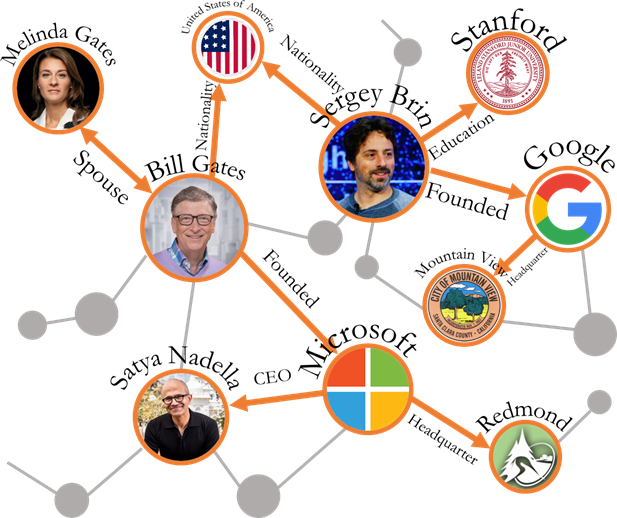
\includegraphics[width=15cm]{images/KGexample1.png}
\caption{Đồ thị tri thức với các thực thể như cá nhân, tổ chức, địa điểm và quốc gia được kết nối qua các mối quan hệ như sáng lập, quốc tịch, học vấn, trụ sở và vai trò lãnh đạo.
Các nút đại diện cho thực thể nổi bật (Bill Gates, Sergey Brin, Microsoft, Google...) và các cạnh có hướng thể hiện rõ ràng loại quan hệ giữa chúng.}
\label{fig:chatbots_classification}
\end{figure}

Mặc dù đồ thị tri thức là một công cụ mạnh mẽ cho việc tổ chức và xử lý kiến thức, chúng thường bị giới hạn trong một không gian tĩnh mà ở đó các nút và cạnh không phát triển theo diễn biến thời gian. Hạn chế này vô tình khiến đồ thị tri thức thiếu đi khả năng phản ánh sự biến đổi của thế giới thực, nơi mà sự liên kết giữa các thực thể có thể được hình thành hay mất đi qua từng thời điểm khác nhau. Ví dụ, quan sát đồ thị tri thức tĩnh trong hình minh họa, ta có thể thấy các mối quan hệ như "Bill Gates - Founded - Microsoft" hoặc "Sergey Brin - Founded - Google" được biểu diễn mà không có thông tin thời gian cụ thể. Điều này dẫn đến việc không thể xác định được rằng Bill Gates thành lập Microsoft vào năm 1975, hay Sergey Brin đồng sáng lập Google vào năm 1996. Hơn nữa, với lượng thông tin ngày càng lớn và phức tạp như hiện tại, việc thiếu yếu tố thời gian khiến cho các hệ thống dựa trên đồ thị tri thức tĩnh không thể nắm bắt được sự thay đổi của các mối quan hệ theo thời gian, dẫn đến thông tin lỗi thời và không chính xác cho các ứng dụng thực tế.

Để giải quyết vấn đề này, đồ thị tri thức thời gian (Temporal Knowledge Graph - TKG)~\cite{ref_article02} được đề xuất với ý tưởng chính là bổ sung một chiều thời gian vào cấu trúc bộ ba (thực thể đầu, quan hệ, thực thể đuôi) ban đầu. Lúc này, bộ ba sẽ mở rộng thành bộ bốn (thực thể đầu, quan hệ, thực thể đuôi, nhãn thời gian) và tri thức được mã hóa thành (Bill Gates, Founded, Microsoft, 1975) hoặc (Sergey Brin, Founded, Google, 1996). Việc tích hợp thêm trường thời gian giúp cho đồ thị tri thức nắm bắt sự thay đổi, mang đến khả năng diễn đạt và xử lý kiến thức một cách linh hoạt hơn, phù hợp hơn với bản chất động của thế giới thực.

\begin{figure}[h!]
\centering
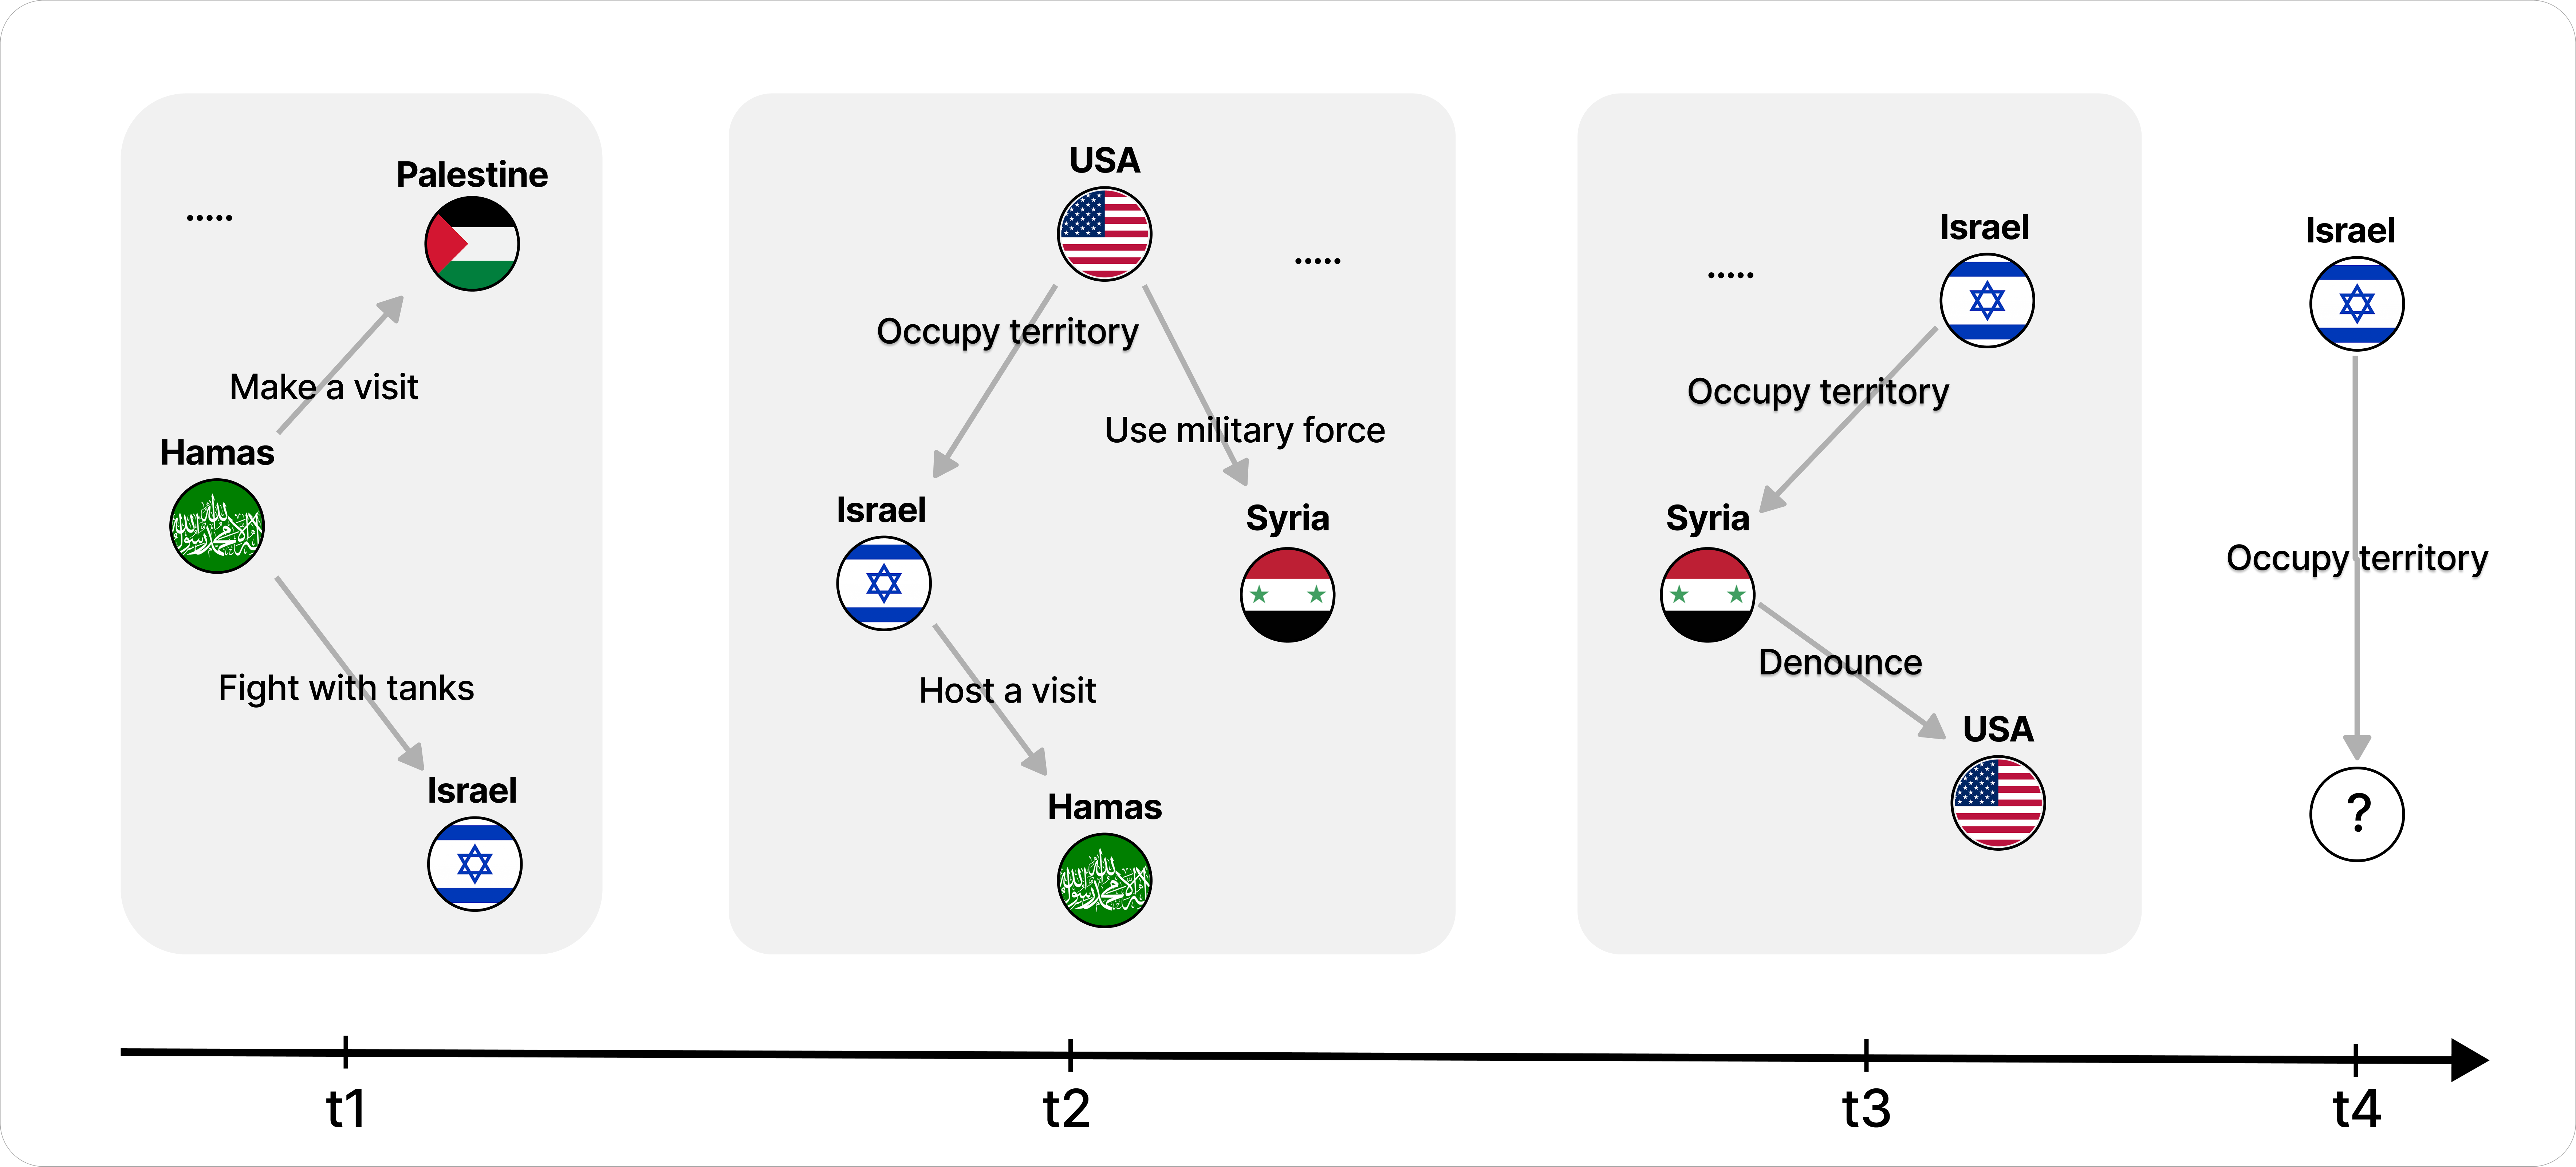
\includegraphics[width=15cm]{images/TKGexample1.png}
\caption{Hình ảnh minh họa quá trình dự đoán sự kiện tương lai trên Đồ thị Tri thức Thời gian (Temporal Knowledge Graph - TKG). Tại mỗi thời điểm $t_1, t_2, t_3$, các sự kiện giữa các thực thể như Israel, Hamas, USA, Syria... được biểu diễn dưới dạng các bộ tứ (subject, relation, object, timestamp). Dựa trên chuỗi sự kiện lịch sử này, mô hình TKGR sẽ sử dụng các quan hệ và tương tác trong quá khứ để dự đoán đối tượng (object) tiếp theo của chủ thể (subject) Israel với quan hệ "Occupy territory" tại thời điểm $t_4$. Quá trình này thể hiện khả năng suy luận và dự báo sự kiện tương lai dựa trên mẫu quan hệ động trong quá khứ của đồ thị tri thức thời gian.}
\label{fig:chatbots_classification}
\end{figure}

Cả đồ thị tri thức tĩnh và đồ thị tri thức thời gian đều được xây dựng từ nhiều nguồn dữ liệu mở với quy mô lớn (ví dụ GDELT, YAGO), tuy nhiên, chúng đều gặp phải vấn đề chung về tính bất hoàn thiện. Tính bất hoàn thiện này thể hiện ở việc các tri thức giá trị trong đồ thị tri thức thời gian thường bị mất đi các thực thể, mối quan hệ, thông tin thời gian hoặc thậm chí là bộ bốn dữ kiện bị ẩn hoàn toàn. Hệ quả là các ứng dụng dưới dòng bị hạn chế về độ chính xác do không thể tạo ra các kết nối quan trọng cho thông tin được truy vấn, dẫn đến các giả định sai lệch so với thực tế.

Bài toán suy luận trên đồ thị tri thức thời gian (Temporal Knowledge Graph Reasoning - TKGR)~\cite{ref_article03} nhằm giải quyết vấn đề này bằng cách dự đoán các sự kiện mới dựa trên thông tin lịch sử có sẵn. Nghiên cứu hiện nay cho thấy rằng các mô hình TKGR có thể được chia làm hai nhánh chính là suy luận dựa trên nội suy và suy luận dựa trên ngoại suy. Với nội suy, các kỹ thuật ở nhánh này dự đoán các dữ kiện mới bằng việc phân tích và khai thác các đặc trưng của dữ kiện đã có trong TKGs, các phương pháp như phân rã ten-xơ (Tensor Decomposition) và chuyển vị quan hệ thời gian (Time-Aware Relation Transformation) nổi bật trong nhánh này do độ chính xác cao. Với ngoại suy, các kỹ thuật sẽ chú trọng vào tính phát triển của dữ liệu qua thời gian để dự đoán các dữ kiện nằm bên ngoài tập dữ liệu, nhằm dự đoán những sự kiện trong tương lai, các hướng giải quyết là mạng nơ-ron đồ thị thời gian (Temporal Graph Neural Networks) và suy tập luật thời gian (Temporal Rule Induction) xuất hiện nhiều trong nghiên cứu gần đây từ nhánh này.

Cả hai nhánh tiếp cận đều có những ưu điểm riêng trong việc tích hợp thông tin thời gian vào mô hình. Tuy nhiên, trong phạm vi của đề tài này, chúng tôi lựa chọn phương pháp tích hợp tri thức đa nguồn trong nhánh tiếp cận ngoại suy để giải quyết bài toán suy luận đồ thị tri thức thời gian. Lý do là phương pháp này có khả năng dự đoán các sự kiện tương lai bằng cách tận dụng sức mạnh của các mô hình ngôn ngữ lớn (LLMs)~\cite{ref_article04} trong việc hiểu ngữ nghĩa và suy luận phức tạp, đồng thời có thể xử lý được các truy vấn linh hoạt theo từng ngữ cảnh cụ thể.

Đặc biệt, sự xuất hiện của các LLMs như GPT~\cite{ref_article05}, LLaMA~\cite{ref_article06}, và DeepSeek~\cite{ref_article07} đã mở ra những cơ hội mới cho TKGR nhờ khả năng xử lý ngữ nghĩa và suy luận vượt trội. Các mô hình này có thể hiểu được các mối liên kết ngữ nghĩa phức tạp và các mẫu thời gian trong dữ liệu, mang lại tiềm năng giải quyết những thách thức về tính giải thích trong TKGR~\cite{ref_article03}. Chính vì vậy, đề tài này tập trung vào việc phát triển phương pháp MSKGen (Multi-Source Knowledge-Based Generation), một cách tiếp cận mới cho TKGR dựa trên việc tích hợp tri thức đa nguồn và tùy chỉnh theo truy vấn, nhằm tận dụng tối đa khả năng của LLMs trong việc dự đoán các sự kiện tương lai một cách chính xác và có tính giải thích cao.


\section{Thách thức của bài toán}

\subsection{Hạn chế trong khai thác ngữ nghĩa của LLMs}
Các phương pháp hiện tại ứng dụng LLMs vào TKGR chủ yếu tập trung vào kỹ thuật prompt engineering đơn giản mà chưa tận dụng hết tiềm năng hiểu ngữ nghĩa sâu của mô hình. Việc phụ thuộc vào các phương pháp truy xuất truyền thống dựa trên khớp lược đồ (schema matching) dẫn đến việc bỏ qua các mối quan hệ ngữ nghĩa tiềm ẩn trong dữ liệu lịch sử. Ví dụ, khi dự đoán sự kiện "công ty A hợp tác với công ty B", các phương pháp hiện tại chỉ xem xét các sự kiện trực tiếp liên quan đến hai công ty này mà không nhận biết được mối liên hệ gián tiếp thông qua các thực thể trung gian hoặc ngữ cảnh thời gian mở rộng. Điều này làm giảm khả năng phát hiện các pattern phức tạp và quan hệ đa tầng trong TKGs.

\subsection{Thiếu tính cá nhân hóa trong suy luận}
Các hệ thống TKGR hiện có thường áp dụng cùng một chiến lược suy luận cho mọi truy vấn mà không xem xét đặc thù ngữ nghĩa của từng yêu cầu cụ thể. Việc không phân biệt được sự khác biệt giữa các loại truy vấn (ví dụ: truy vấn về sự kiện kinh tế vs. sự kiện chính trị) dẫn đến việc tạo ra các phản hồi chung chung. Hệ quả là các dự đoán thiếu tính chính xác cục bộ và không phản ánh được sắc thái thời gian đặc thù của từng sự kiện. Nghiêm trọng hơn, các phương pháp dựa trên LLMs hiện tại thường không xử lý được các truy vấn yêu cầu kết hợp nhiều nguồn tri thức đa dạng.

\subsection{Khó khăn trong xử lý thông tin thời gian đa tầng}
TKGs chứa các mối quan hệ thời gian ở nhiều mức độ phức tạp khác nhau, từ các sự kiện đơn lẻ (event-level) đến các xu hướng dài hạn (trend-level). Các phương pháp hiện tại gặp khó khăn trong việc đồng thời xử lý:
\begin{itemize}
    \item Thông tin lịch sử bậc cao (high-order dependencies) giữa các sự kiện cách biệt về thời gian
    \item Tương tác phi tuyến tính giữa các yếu tố thời gian ngắn hạn và dài hạn
    \item Sự mâu thuẫn tiềm ẩn giữa các nguồn tri thức khác nhau
\end{itemize}

\subsection{Giới hạn trong tích hợp tri thức đa nguồn}
Phần lớn các phương pháp TKGR hiện nay chỉ tập trung vào khai thác thông tin từ cấu trúc đồ thị mà bỏ qua các nguồn tri thức bổ sung như văn bản phi cấu trúc, cơ sở dữ liệu quan hệ, hay tri thức miền chuyên gia. Sự thiếu hụt này dẫn đến hai hệ quả chính: (1) Các dự đoán không thể tận dụng được thông tin ngữ cảnh phong phú từ các nguồn dữ liệu đa phương thức, (2) Hệ thống khó duy trì tính nhất quán khi xử lý các truy vấn đòi hỏi tích hợp tri thức liên ngành.

\subsection{Thách thức về tính giải thích}
Mặc dù LLMs có khả năng suy luận phức tạp, các phương pháp TKGR hiện tại chưa cung cấp được cơ chế giải thích rõ ràng cho từng dự đoán. Việc thiếu minh bạch trong quá trình ra quyết định đặc biệt nghiêm trọng trong các ứng dụng nhạy cảm như dự báo tài chính hoặc chẩn đoán y tế, nơi cần theo dõi được logic suy luận và nguồn gốc của từng dự đoán. Hơn nữa, sự phụ thuộc quá mức vào các mô hình hộp đen (black-box models) làm hạn chế khả năng hiệu chỉnh và tối ưu hệ thống.


\section{Động lực và hướng tiếp cận}

\subsection{Động lực nghiên cứu}
Các phương pháp hiện tại trong suy luận đồ thị tri thức thời gian (TKGR) chủ yếu dựa trên các mô hình học sâu với ba hạn chế chính: (1) Thiếu tính giải thích do sử dụng kiến trúc "hộp đen", (2) Phụ thuộc quá mức vào thông tin lịch sử bậc nhất mà bỏ qua các mối quan hệ đa tầng, và (3) Khả năng tùy biến thấp trước các truy vấn cụ thể. Ví dụ, khi dự đoán sự kiện "Công ty A hợp tác chiến lược với Công ty B", các phương pháp truyền thống chỉ xem xét các sự kiện trực tiếp giữa hai thực thể này mà bỏ qua các yếu tố ngữ cảnh như mối quan hệ gián tiếp qua đối tác phụ hoặc xu hướng dài hạn trong lịch sử hợp tác.

Sự xuất hiện của các mô hình ngôn ngữ lớn (LLMs) mở ra cơ hội cải thiện TKGR thông qua khả năng hiểu ngữ nghĩa sâu và suy luận logic. Tuy nhiên, việc áp dụng LLMs vào TKGR hiện nay vẫn chưa khai thác hết tiềm năng do: (1) Chiến lược prompt đơn giản không tận dụng được cấu trúc thời gian phức tạp, (2) Thiếu cơ chế tích hợp tri thức từ nhiều nguồn đa dạng, và (3) Không cân bằng được giữa độ chính xác và tính giải thích. Điều này dẫn đến các dự đoán thiếu tin cậy trong các ứng dụng thực tế như dự báo tài chính hoặc phân tích chính trị.

\subsection{Hướng tiếp cận}
Phương pháp MSKGen được thiết kế để giải quyết các thách thức trên thông qua ba trụ cột chính:

1. \textbf{Trích xuất tri thức dựa trên quy tắc thời gian}: Sử dụng kỹ thuật "temporal random walks" để khám phá các mẫu quan hệ động trong dữ liệu lịch sử. Quy trình bao gồm: (a) Lấy mẫu các chuỗi sự kiện tuân thủ ràng buộc thời gian, (b) Đánh giá chất lượng quy tắc bằng độ đo Kulczynski, (c) Tinh chỉnh quy tắc thông qua tương tác với LLMs. Ví dụ, từ chuỗi sự kiện "A hợp tác với B → B đầu tư vào C → C mở rộng thị trường", hệ thống có thể rút ra quy tắc logic về chuỗi tác động kinh tế.

2. \textbf{Truy xuất tri thức ngữ nghĩa đa nguồn}: Áp dụng kỹ thuật RAG để tích hợp: (a) Dữ liệu có cấu trúc từ đồ thị tri thức, (b) Văn bản phi cấu trúc từ báo cáo/bài nghiên cứu, (c) Tri thức chuyên gia được vector hóa. Hệ thống sử dụng cơ sở dữ liệu vector Chroma để tìm kiếm các sự kiện tương đồng ngữ nghĩa, cho phép phát hiện các mối quan hệ tiềm ẩn không được biểu diễn tường minh trong đồ thị.

3. \textbf{Lập luận đa nguồn có hướng dẫn}: Kết hợp đầu ra từ hai quy trình trên thông qua cơ chế điều phối động: (a) Phân tích cú pháp và ngữ nghĩa của truy vấn để xác định trọng số cho từng nguồn tri thức, (b) Sử dụng LLMs để tổng hợp thông tin dưới dạng các chuỗi suy luận có cấu trúc, (c) Đánh giá độ tin cậy dựa trên sự nhất quán giữa các nguồn. Ví dụ, khi dự đoán xu hướng thị trường, hệ thống sẽ cân bằng giữa quy tắc thống kê từ dữ liệu lịch sử và phân tích ngữ cảnh từ báo cáo kinh tế.

Khác biệt cốt lõi của MSKGen so với các phương pháp trước đây nằm ở khả năng thích ứng động với từng truy vấn cụ thể thông qua việc tích hợp: (1) Logic thời gian từ các quy tắc được học, (2) Bối cảnh ngữ nghĩa từ RAG, và (3) Khả năng suy luận đa tầng của LLMs. Sự kết hợp này không chỉ cải thiện độ chính xác mà còn tạo ra các lộ trình suy luận có thể giải thích được, đáp ứng yêu cầu của các ứng dụng thực tế yêu cầu tính minh bạch cao.

\section{Mục tiêu và đóng góp của đề tài}

\subsection{Mục tiêu đề tài}
Mục tiêu chung của đề tài khóa luận tốt nghiệp này là nghiên cứu và phát triển phương pháp suy luận hiệu quả trên đồ thị tri thức thời gian ở nhánh bài toán ngoại suy, tập trung vào việc dự đoán các sự kiện tương lai dựa trên chuỗi sự kiện lịch sử. Mục tiêu cụ thể bao gồm:

• Tổng hợp và phân tích các công trình nghiên cứu trong và ngoài nước về bài toán suy luận đồ thị tri thức thời gian, đặc biệt là các phương pháp ứng dụng mô hình ngôn ngữ lớn vào TKGR nhằm khảo sát các xu hướng và tiến triển của lĩnh vực.

• Phân tích sâu các thách thức và hạn chế của các phương pháp hiện tại trong việc tích hợp tri thức đa nguồn và tùy chỉnh suy luận theo truy vấn cụ thể. Từ đó đề xuất hướng giải quyết khả quan cho nhánh bài toán ngoại suy thông qua việc kết hợp kỹ thuật trích xuất quy tắc và truy xuất ngữ nghĩa.

• Thiết kế và triển khai framework MSKGen, một phương pháp mới tích hợp tri thức từ nhiều nguồn khác nhau để nâng cao độ chính xác và tính giải thích trong dự đoán sự kiện tương lai trên đồ thị tri thức thời gian.

• Thực nghiệm và đánh giá hiệu suất của mô hình MSKGen trên các bộ dữ liệu chuẩn, so sánh với các phương pháp tiên tiến hiện có để chứng minh tính hiệu quả và khả năng ứng dụng thực tế của phương pháp đề xuất.

\subsection{Đóng góp của đề tài}
Những đóng góp chính của đề tài nghiên cứu này bao gồm:

• Giới thiệu MSKGen, một framework tiên tiến cho suy luận đồ thị tri thức thời gian theo truy vấn cụ thể thông qua tích hợp tri thức đa nguồn. Phương pháp này kết hợp khả năng trích xuất quy tắc logic chất lượng cao từ dữ liệu lịch sử với kỹ thuật truy xuất ngữ nghĩa, đảm bảo cả tính chính xác lẫn độ sâu ngữ nghĩa trong quá trình suy luận.

• Phát triển cơ chế suy luận nhận biết truy vấn (query-aware reasoning) có khả năng tùy chỉnh quá trình dự đoán theo đặc thù của từng yêu cầu cụ thể. Cơ chế này tận dụng kỹ thuật Retrieval-Augmented Generation để thu thập ngữ cảnh phong phú từ các nguồn dữ kiện đa dạng, nâng cao chất lượng và độ tin cậy của dự đoán.

• Tối ưu hóa khả năng xử lý của mô hình ngôn ngữ lớn trong việc kết nối các dữ kiện có cấu trúc đa dạng và tích hợp thông tin tương tự về mặt ngữ nghĩa. Điều này cho phép MSKGen tạo ra các câu trả lời phù hợp với từng truy vấn cụ thể trong khi tối đa hóa tiềm năng hiểu ngữ nghĩa của LLMs.

• Đánh giá toàn diện trên các tập dữ liệu chuẩn cho thấy MSKGen vượt trội đáng kể so với các phương pháp hiện có về độ chính xác dự đoán sự kiện, đồng thời duy trì tính giải thích cao thông qua việc kết hợp tri thức từ nhiều nguồn khác nhau.

\subsection{Bố cục trình bày}
Khóa luận được tổ chức thành sáu chương với các nội dung được tóm tắt như sau:

• Chương 1: Trình bày tổng quan về vấn đề đang được nghiên cứu, bao gồm giới thiệu về đồ thị tri thức thời gian và bài toán suy luận TKGR. Chương này phân tích các thách thức hiện tại của bài toán, từ đó chỉ ra động lực, hướng tiếp cận, mục tiêu cũng như đóng góp của khóa luận.

• Chương 2: Tập trung vào việc khảo sát và phân tích các công trình nghiên cứu liên quan đến suy luận đồ thị tri thức thời gian, đặc biệt là các phương pháp ứng dụng mô hình ngôn ngữ lớn. Thông qua phân tích ưu điểm và hạn chế của từng phương pháp, chương này làm rõ cơ sở lựa chọn hướng tiếp cận của nghiên cứu.

• Chương 3: Cung cấp nền tảng lý thuyết và các khái niệm cơ bản làm cơ sở cho phương pháp đề xuất. Nội dung bao gồm định nghĩa chính thức về đồ thị tri thức thời gian, bài toán suy luận TKGR, các kỹ thuật mô hình ngôn ngữ lớn và Retrieval-Augmented Generation.

• Chương 4: Giới thiệu chi tiết framework MSKGen, bao gồm kiến trúc tổng thể, các thành phần chính và cơ chế hoạt động. Chương này trình bày phương pháp trích xuất quy tắc thời gian, kỹ thuật truy xuất ngữ nghĩa và cơ chế suy luận tích hợp đa nguồn.

• Chương 5: Trình bày kết quả thực nghiệm toàn diện của MSKGen trên các tập dữ liệu chuẩn, so sánh hiệu suất với các phương pháp tiên tiến hiện có. Chương này cũng phân tích ảnh hưởng của các siêu tham số và thành phần khác nhau đến hiệu suất của mô hình.

• Chương 6: Tóm tắt các kết quả đạt được, đánh giá mức độ hoàn thành mục tiêu đề ra và đề xuất các hướng nghiên cứu tiềm năng trong tương lai dựa trên những hạn chế và cơ hội mở ra từ nghiên cứu này.
